\documentclass[12pt,a4paper]{article}
%\usepackage[utf8]{vietnam}
\usepackage[margin=2.5cm]{geometry}
\usepackage{amsmath}
\usepackage{graphicx}
\usepackage{float}
\usepackage{array}
\usepackage{booktabs}
\usepackage{hyperref}
\usepackage{fancyhdr}
\usepackage{lastpage}
\usepackage{caption}
\usepackage{subcaption}
\usepackage{tikz}
\usepackage{pgfplots}
\usepackage{enumitem}
\pgfplotsset{compat=1.18}
\usepackage{tabularx}
\setlist[itemize]{leftmargin=*,itemsep=3pt,topsep=4pt}
\setlist[enumerate]{leftmargin=*,itemsep=4pt,topsep=4pt}

% Thiết lập header và footer
\pagestyle{fancy}
\fancyhf{}
\setlength{\headheight}{38pt}

\fancyhead[L]{%
	\begin{minipage}[c]{1.6cm}
		
\includegraphics[height=1.1cm]{01_logobachkhoasang.png}
	\end{minipage}%
	\hspace{0.15cm}%
	\begin{minipage}[c]{0.72\textwidth}
		\small
		Trường Đại học Bách khoa - ĐHQG-HCM\\
		Khoa Khoa học và Kỹ thuật Máy tính
	\end{minipage}%
}
\fancyhead[R]{}
\renewcommand{\headrulewidth}{0.5pt}
\usepackage{listings}
\usepackage{xcolor}

\lstset{
    basicstyle=\ttfamily\small,
    keywordstyle=\color{blue},
    commentstyle=\color{gray},
    frame=single,
    breaklines=true,
    columns=fullflexible,
    keepspaces=true
}
\fancyfoot[L]{\small\textit{Báo cáo Bài tập lớn Hệ điều hành (TN)}}
\fancyfoot[R]{\small\textbf{Trang \thepage/\pageref{LastPage}}}
\renewcommand{\footrulewidth}{0.5pt}

% Thiết lập cho trang title
\fancypagestyle{titlepage}{
	\fancyhf{}
	\renewcommand{\headrulewidth}{0pt}
	\renewcommand{\footrulewidth}{0pt}
}

% ===========================================================
% Ô GIỮ CHỖ: in chữ xám, ghi người viết và việc cần viết.
% Viết xong phần nào thì XÓA dòng \viet{...}{...} của phần đó.
% ===========================================================
\newcommand{\viet}[2]{\par\noindent\textcolor{gray}{\textit{[#1] #2}}\par\medskip}

\begin{document}

	%========================= TITLE PAGE =========================
	\begin{titlepage}
		\centering

		{\large ĐẠI HỌC QUỐC GIA THÀNH PHỐ HỒ CHÍ MINH\\}
		{\large TRƯỜNG ĐẠI HỌC BÁCH KHOA\\}

		
\includegraphics[width=0.65\linewidth]{01_logobachkhoasang.png}\\[0.5cm]

		{\large \textbf{HỆ ĐIỀU HÀNH (THÍ NGHIỆM) - CO2018}\\[0.3cm]}

		\noindent\makebox[\textwidth]{\rule{16cm}{0.4pt}}
		{\LARGE \textbf{BÁO CÁO}\\}
		{\LARGE \textbf{BÀI TẬP LỚN - ossim\_demacOprx}}\\
		\noindent\makebox[\textwidth]{\rule{16cm}{0.4pt}}

		{\large GVHD: Nguyễn Tuấn Huy\\[1.2cm]}

		{\large Lớp: L01 \quad Nhóm: 08\\[0.6cm]}

		{\large\begin{center}
			\begin{tabular}{>{\bfseries}c c}
				Hoàng Phạm Tiến Thành & 2413148 \\
				Trần Duy Nhân & 2412439 \\
				Đặng Bá Khôi & 2411679 \\
				Huỳnh Nguyễn Yến Linh & 2411871 \\
			\end{tabular}
		\end{center}
		}
		\vfill
		{\large TP. Hồ Chí Minh, tháng 11 năm 2026}

	\end{titlepage}

	\tableofcontents

	% ===========================================================
	% LỜI MỞ ĐẦU — KHÔI
	% ===========================================================
	\clearpage
	\section*{Lời Mở Đầu}
	\addcontentsline{toc}{section}{Lời Mở Đầu}

	Hệ điều hành là thành phần quan trọng giúp quản lý tài nguyên phần cứng và điều phối hoạt động của các chương trình. Những kiến thức như lập lịch CPU, quản lý bộ nhớ, phân trang hay đồng bộ hóa sẽ dễ hiểu hơn khi được áp dụng vào một chương trình mô phỏng cụ thể. Trong khuôn khổ môn học Hệ điều hành (CO2018), nhóm chúng em thực hiện bài tập lớn \texttt{ossim\_demacOprx} dựa trên mã nguồn được cung cấp và các yêu cầu của học kỳ HK261. Mục tiêu của nhóm không chỉ là hoàn thiện các chức năng được giao mà còn là tìm hiểu cách chúng phối hợp với nhau trong quá trình thực thi. Qua việc đọc mã nguồn, chỉnh sửa từng thành phần, biên dịch và chạy các trường hợp kiểm thử, nhóm có cơ hội tiếp cận gần hơn với những vấn đề thực tế khi xây dựng một hệ điều hành, đặc biệt là việc quản lý trạng thái tiến trình và tài nguyên dùng chung.

	Trong bài tập lớn này, nhóm tập trung vào một số nội dung chính. Bộ lập lịch \textit{Multi-Level Queue} (MLQ) tổ chức tiến trình theo các hàng đợi ưu tiên và phân phối lượt chạy trên một hoặc nhiều CPU. Phần quản lý bộ nhớ được mở rộng với bố cục không gian địa chỉ kiểu macOS, cấp phát theo vùng, phân trang đa cấp và cơ chế hoán đổi trang khi cần thiết. Bên cạnh đó, hệ thống mô phỏng sự tách biệt giữa không gian người dùng và không gian nhân, cùng phương thức giao tiếp thông qua các lời gọi hệ thống. Một nội dung
	đáng chú ý là cơ chế co-processor DMA hoạt động bất đồng bộ: sau khi gửi yêu cầu truyền dữ liệu, CPU có thể tiếp tục thực thi tiến trình khác; khi DMA hoàn tất, thông báo ngắt được chuyển đến CPU để xử lý. Nhóm cũng chú trọng việc giữ lại tài nguyên của tiến trình nếu DMA vẫn đang sử dụng, nhằm tránh giải phóng bộ nhớ quá sớm.

	Báo cáo trình bày cách tổ chức và hiện thực các thành phần trên, đồng thời đối chiếu với kết quả chạy từ phiên bản mã nguồn đã tích hợp của nhóm. Qua quá trình thực hiện, nhóm rèn luyện thêm kỹ năng đọc hiểu chương trình C/C++, phối hợp thay đổi mã nguồn và kiểm tra lỗi trên môi trường Linux. Chúng em xin chân thành cảm ơn thầy Nguyễn Tuấn Huy đã giảng dạy, hướng dẫn và góp ý để nhóm có thể hoàn thành bài tập lớn này. Dù đã cố gắng, báo cáo khó tránh khỏi thiếu sót; nhóm rất mong nhận được thêm nhận xét để có thể hoàn thiện kiến thức và cách triển khai trong thời gian tới.

	% Bắt đầu nội dung chính ở trang mới, không chung trang với Lời mở đầu.
	\clearpage

	% ===========================================================
	% 1. GIỚI THIỆU VÀ PHÂN CÔNG — KHÔI
	% ===========================================================
	\section{Giới thiệu và phân công}

	\subsection{Môi trường và cách chạy}
	\begin{itemize}
	    \item \textbf{Nền tảng:} Ubuntu/Linux; mã nguồn C/C++.
	    \item \textbf{Công cụ:} Makefile, GCC/G++, thư viện \texttt{pthread} và Verilator cho DMA RTL.
	    \item \textbf{Cấu hình:} \texttt{MLQ\_SCHED}, \texttt{MM\_PAGING}, \texttt{MM64} bật trong \texttt{include/os-cfg.h}; \texttt{MAX\_PRIO = 140}.
	    \item \textbf{Cách chạy:} truyền tên cấu hình trong \texttt{input/} cho chương trình \texttt{os}.
	\end{itemize}

	\begin{lstlisting}[language=bash]
make clean
make os
./os sched
./os sched_0
./os sched_1
./os khoi_dma_nonblocking_test
./os khoi_dma_deferred_test
	\end{lstlisting}

	\subsection{Phân công công việc}
	\begin{table}[H]
	\centering\small
	\begin{tabularx}{\linewidth}{|l|c|X|}
	\hline
	\textbf{Thành viên} & \textbf{MSSV} & \textbf{Phần phụ trách} \\
	\hline
	Hoàng Phạm Tiến Thành & 2413148 & Swapping, bộ nhớ kernel, giao tiếp user/kernel và cầu nối DMA đa trang. \\
	\hline
	Trần Duy Nhân & 2412439 & \textcolor{gray}{\textit{[Nhân] Điền phần code và phần báo cáo phụ trách}} \\
	\hline
	Đặng Bá Khôi & 2411679 & Scheduling, xử lý ngắt và DMA bất đồng bộ. \\
	\hline
	Huỳnh Nguyễn Yến Linh & 2411871 & \textcolor{gray}{\textit{[Linh] Điền phần code và phần báo cáo phụ trách}} \\
	\hline
	\end{tabularx}
	\caption{Phân công công việc của nhóm}
	\end{table}

	% ===========================================================
	% 2. SCHEDULER — KHÔI
	% ===========================================================
	\section{Scheduling}
	\subsection{Hiện thực MLQ}

	\noindent\textbf{Cấu trúc quản lý tiến trình:}
	\begin{itemize}
	    \item \texttt{mlq\_ready\_queue[MAX\_PRIO]}: mỗi mức ưu tiên có một hàng đợi riêng.
	    \item \texttt{running\_list}: lưu các PCB đang được CPU xử lý.
	    \item \texttt{current\_prio}: mức ưu tiên hiện tại của bộ chọn MLQ.
	    \item \texttt{slot[p]}: số lượt chọn còn lại của mức ưu tiên \(p\), khởi tạo bằng \(\texttt{MAX\_PRIO}-p\).
	\end{itemize}

	\noindent\textbf{Các thao tác hàng đợi trong \texttt{src/queue.c}:}
	\begin{itemize}
	    \item \texttt{enqueue()}: đưa PCB vào cuối hàng đợi.
	    \item \texttt{dequeue()}: lấy PCB đầu hàng đợi, bảo đảm nguyên tắc FIFO.
	    \item \texttt{purgequeue()}: xóa một PCB xác định khỏi hàng đợi.
	\end{itemize}

	\noindent\textbf{Các bước chọn tiến trình trong \texttt{src/sched.c}:}
	\begin{enumerate}
	    \item \texttt{add\_mlq\_proc()} đưa PCB mới vào queue theo \texttt{proc->prio}.
	    \item \texttt{get\_mlq\_proc()} bắt đầu duyệt từ \texttt{current\_prio}.
	    \item Nếu queue không rỗng và \texttt{slot[p] > 0}, lấy PCB, thêm vào \texttt{running\_list}, giảm \texttt{slot[p]}.
	    \item Khi không chọn được tiến trình trong một lượt quét, khởi tạo lại quota và thử thêm một lượt.
	    \item Hết time slice, \texttt{put\_mlq\_proc()} trả PCB về queue; kết thúc tiến trình thì \texttt{finish\_proc()} gỡ khỏi \texttt{running\_list}.
	\end{enumerate}

	\noindent\textbf{Time slice và đồng bộ:}
	\begin{itemize}
	    \item Trong \texttt{cpu\_routine()}, mỗi lần \texttt{run(proc)} hoàn thành sẽ giảm \texttt{time\_left} một đơn vị.
	    \item Khi hết lượt chạy, CPU chọn lại tiến trình. \texttt{time\_left} khác với quota \texttt{slot[p]} của MLQ.
	    \item \texttt{queue\_lock} bảo vệ các thao tác với hàng đợi, \texttt{running\_list}, và trạng thái chọn queue khi nhiều CPU cùng chạy.
	\end{itemize}

	\subsection{Biểu đồ Gantt}
	Ba cấu hình sau chạy trên code tích hợp và đều kết thúc với mã thoát 0.
	\begin{table}[H]
	\centering\small
	\begin{tabular}{lrrr}
	\toprule
	\textbf{Input} & \textbf{Quantum} & \textbf{CPU} & \textbf{Tiến trình} \\
	\midrule
	\texttt{sched} & 4 & 2 & 4 \\
	\texttt{sched\_0} & 2 & 1 & 4 \\
	\texttt{sched\_1} & 2 & 1 & 5 \\
	\bottomrule
	\end{tabular}
	\caption{Cấu hình các test lập lịch}
	\label{tab:khoi-sched-config}
	\end{table}

	\noindent\textbf{Test \texttt{sched}:}
	\begin{itemize}
	    \item CPU 1 nhận PID 1 tại slot 1; CPU 0 nhận PID 2 tại slot 2.
	    \item Các CPU tiếp tục phân chia lượt xử lý giữa các PID còn lại.
	    \item Bốn tiến trình đều kết thúc, cho thấy việc dispatch trên 2 CPU.
	\end{itemize}
	\begin{figure}[H]
	    \centering
	    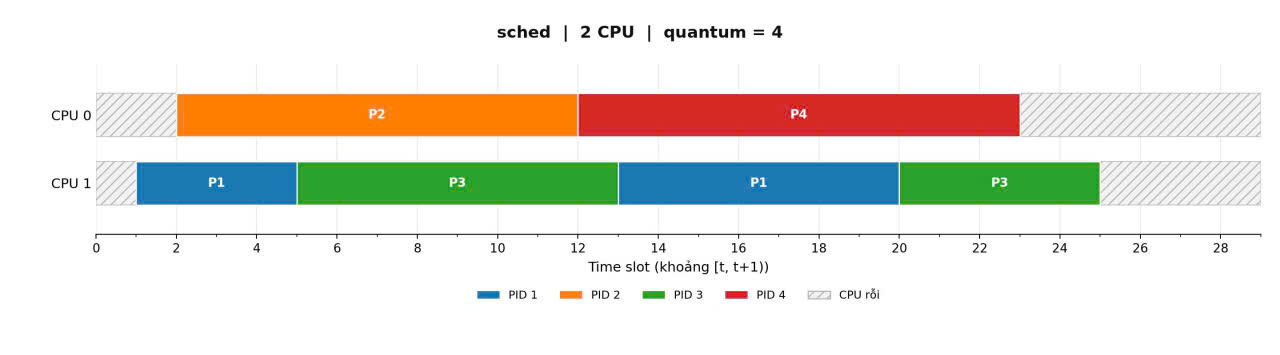
\includegraphics[width=\linewidth]{figures/khoi_sched_gantt.png}
	    \caption{sched -- 2 CPU, quantum = 4}
	    \label{fig:khoi-sched}
	\end{figure}

	\noindent\textbf{Test \texttt{sched\_0}:}
	\begin{itemize}
	    \item PID 1 và PID 2 có cùng mức ưu tiên 4; luân phiên theo quantum 2.
	    \item PID 3 và PID 4 đến sau, được chọn khi nhóm PID đầu đã kết thúc.
	    \item Log thể hiện rõ thao tác \texttt{put\_proc()} và chọn lại tiến trình.
	\end{itemize}
	\begin{figure}[H]
	    \centering
	    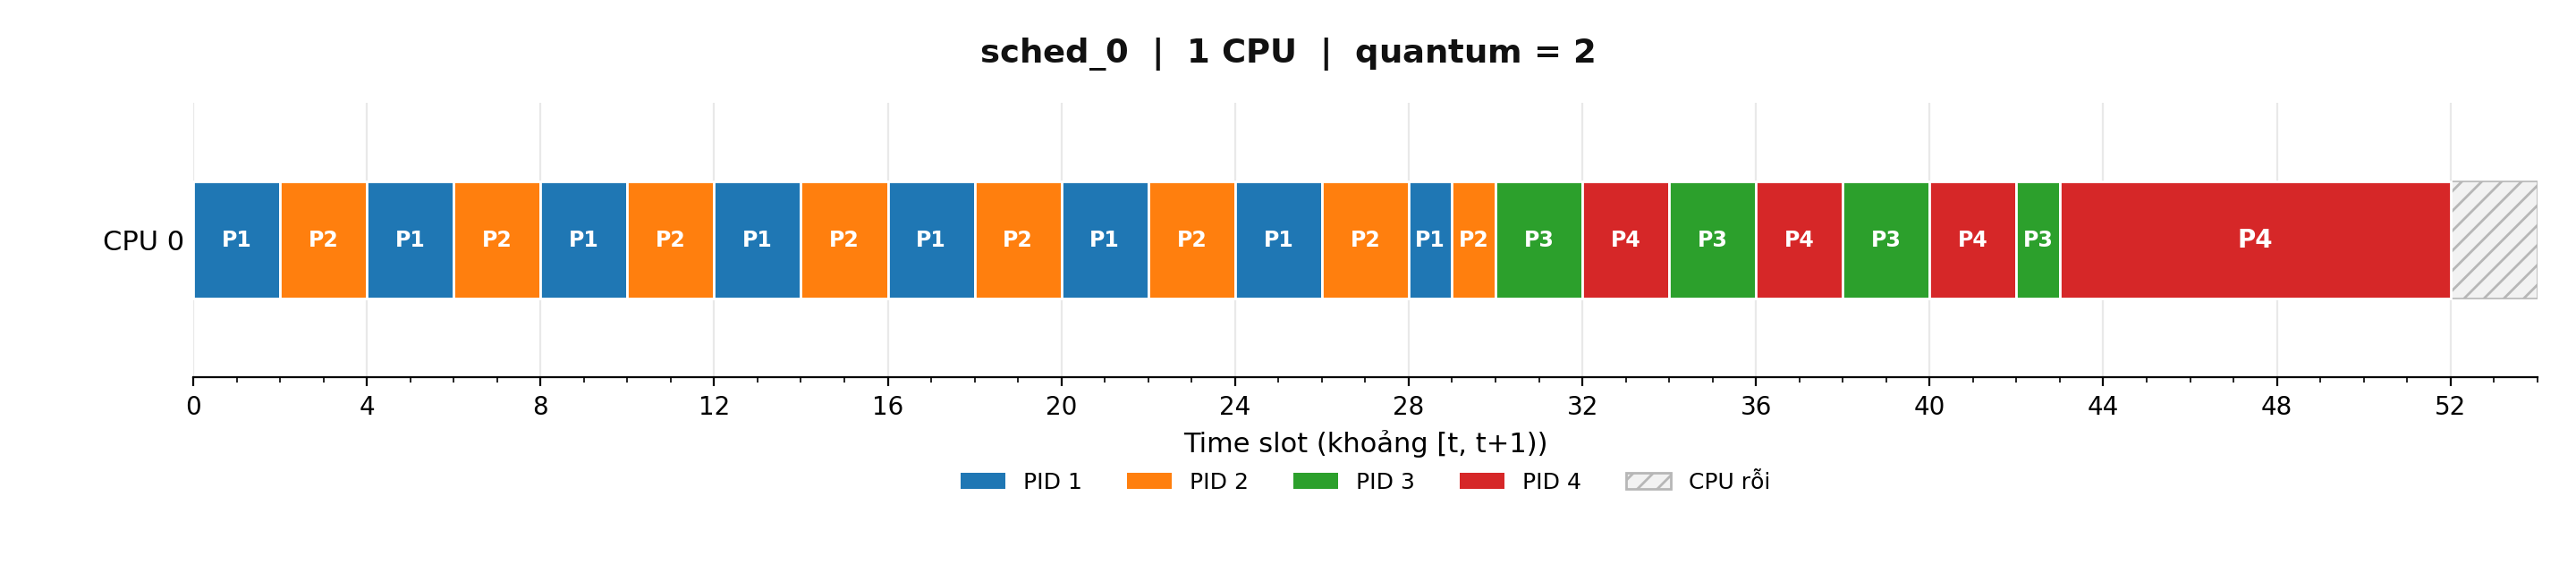
\includegraphics[width=\linewidth]{figures/khoi_sched_0_gantt.png}
	    \caption{sched\_0 -- 1 CPU, quantum = 2}
	    \label{fig:khoi-sched0}
	\end{figure}

	\noindent\textbf{Test \texttt{sched\_1}:}
	\begin{itemize}
	    \item PID 1 liên tục được chọn lại cho đến khi kết thúc ở slot 15.
	    \item PID 2--5 sau đó luân phiên theo quantum 2.
	    \item Quan sát cho thấy độ trễ chờ có thể lớn dù tiến trình đã được nạp.
	\end{itemize}
	\begin{figure}[H]
	    \centering
	    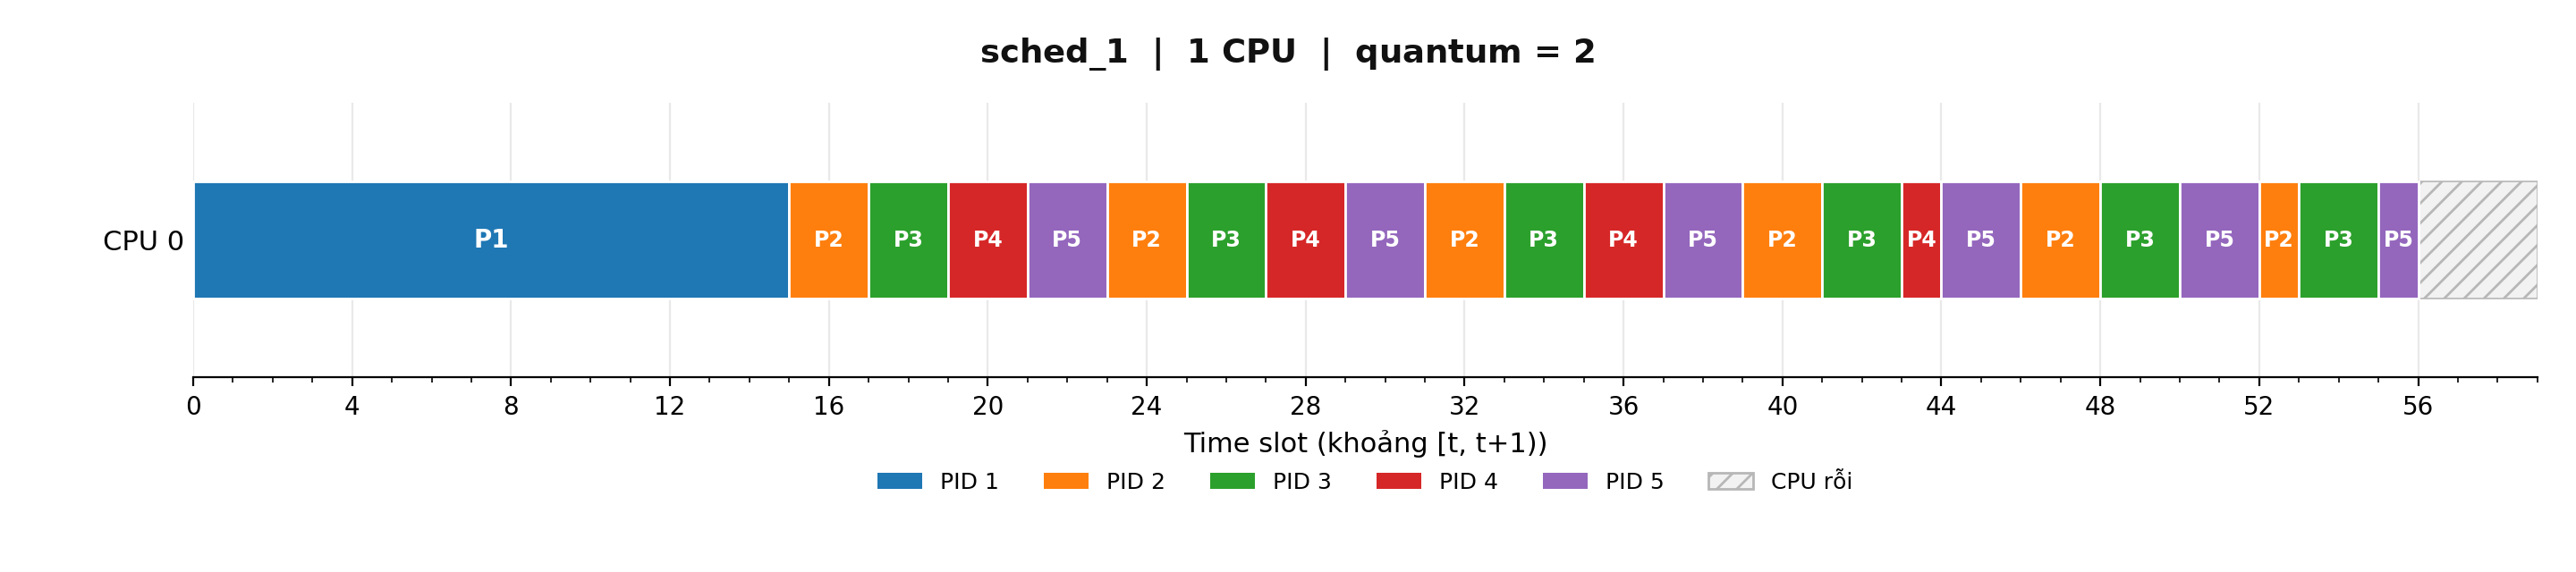
\includegraphics[width=\linewidth]{figures/khoi_sched_1_gantt.png}
	    \caption{sched\_1 -- 1 CPU, quantum = 2}
	    \label{fig:khoi-sched1}
	\end{figure}

	\noindent\textit{Ghi chú:} các thanh PID được xác định từ các dòng \texttt{Time slot}, \texttt{Dispatched process}, \texttt{Put process} và \texttt{Processed ... has finished}. Nhiều lần dispatch lại cùng PID liên tiếp được thể hiện thành một khoảng. Với 2 CPU, các dòng log có thể xen kẽ do chạy song song.

	\subsection{Trả lời câu hỏi}
	\begin{enumerate}
     \item \textbf{Q2 -- When a system call executes too long time, how does the Operating system detect and handle the case?}
	    \begin{itemize}
	        \item Hệ điều hành thực: có thể dùng timer, timeout, watchdog hoặc cơ chế hủy tác vụ phù hợp; không nên tùy tiện ngắt mã kernel đang giữ khóa.
	        \item Simulator hiện tại: \texttt{time\_left} được giảm \emph{sau mỗi lần} \texttt{run(proc)} trở về; hết quantum, CPU gọi \texttt{put\_proc()} để chọn lại.
	        \item Giới hạn: time slice không phải watchdog để cưỡng bức ngắt một system call không trả về.
	        \item Với DMA: request được giao cho \texttt{co\_processor()}; CPU tiếp tục chạy và xử lý completion tại \texttt{dma\_handle\_pending\_irqs()} sau tín hiệu \texttt{SIGUSR1}.
	    \end{itemize}
        
	    \item \textbf{Q3 -- Considering the impactness of MLQ detailed policies, what is the benefit of each policy?}
	    \begin{itemize}
	        \item Nhiều queue ưu tiên: phân loại tiến trình thành các nhóm điều phối khác nhau.
	        \item FIFO trong mỗi queue: tiến trình cùng mức được phục vụ theo thứ tự chờ.
	        \item Đưa về queue khi hết quantum: tạo cơ hội luân phiên giữa các PCB cùng mức.
	        \item Quota \texttt{slot[p]}: phân bổ lượt chọn giữa các mức ưu tiên.
	        \item Liên hệ kết quả: \texttt{sched\_0} thể hiện PID 1/2 luân phiên; \texttt{sched\_1} cho thấy tiến trình đến sau có thể chờ lâu. Do đó không khẳng định MLQ có ưu tiên tức thời hay không starvation trong mọi trường hợp.
	    \end{itemize}
	\end{enumerate}

	% ===========================================================
	% 3. MEMORY LAYOUT KIỂU MACOS — NHÂN
	% ===========================================================
	\section{Memory Layout}

	\subsection{Bố cục vùng nhớ}
	\viet{Nhân}{Bảng layout theo kiểu macOS: PAGEZERO, vùng Small, Medium, Large, vùng kernel (\texttt{KERNEL\_BASE\_ADDR}). Mỗi dòng ghi địa chỉ bắt đầu, kết thúc, kích thước, căn chỉnh, mô tả.}
	\begin{table}[H]
	\centering\small
	\begin{tabularx}{\linewidth}{|l|l|l|l|X|}
	\hline
	\textbf{Vùng} & \textbf{Bắt đầu} & \textbf{Kết thúc} & \textbf{Kích thước} & \textbf{Mô tả} \\
	\hline
	 & & & & \\
	\hline
	\end{tabularx}
	\caption{Bố cục bộ nhớ ảo của một tiến trình}
	\label{tab:memory_layout}
	\end{table}

	\subsection{Lý do thiết kế}
	\viet{Nhân}{Vì sao chia 3 vùng theo kích thước (tham khảo bảng macOS trang 31 của đề), vì sao chọn ngưỡng 512 B / 4096 B và căn chỉnh 16 B / 256 B / 4096 B, lợi ích cho DMA. So sánh ngắn với layout Linux của học kỳ trước.}

	% ===========================================================
	% 4. QUẢN LÝ BỘ NHỚ ẢO — LINH
	% ===========================================================
	\section{Virtual Memory Management}

	\subsection{ALLOC và FREE}
	\viet{Linh}{Luồng ALLOC: tìm vùng trống trong \texttt{vm\_freerg\_list}, không có thì nới \texttt{sbrk} qua \texttt{inc\_vma\_limit}, map trang. Luồng FREE: trả vùng vào danh sách vùng trống.}

	\subsection{Phân vùng theo kích thước}
	\viet{Linh}{\texttt{liballoc} chọn vùng Small, Medium, Large theo size, làm tròn căn chỉnh; \texttt{libfree}, \texttt{libread}, \texttt{libwrite} lấy \texttt{vmaid} từ \texttt{symrgtbl}; \texttt{\_\_free} chỉ chặn khi frame của vùng đang bị DMA ghim.}

	\subsection{Trạng thái cấp phát}
	\viet{Linh}{Bảng hoặc hình trạng thái các vùng sau từng lệnh alloc/free của một test chạy trên bản code cuối.}

	\subsection{Trả lời câu hỏi}
	\begin{enumerate}
	    \item \textbf{What is the primary motivation for combining segmentation with paging in memory management? How does this hybrid approach address limitations inherent in using either technique alone?}
	    \viet{Linh}{Trả lời Q4, liên hệ VMA (phân đoạn) + bảng trang (phân trang) trong code.}

	    \item \textbf{What are the advantages and disadvantages of paging and contiguous memory allocation?}
	    \viet{Linh}{Trả lời Q6.}
	\end{enumerate}

	% ===========================================================
	% 5. PHÂN TRANG ĐA CẤP — NHÂN
	% ===========================================================
	\section{Multi-level Paging}

	\subsection{Sơ đồ phân giải địa chỉ}
	\viet{Nhân}{Cấu trúc địa chỉ 5 cấp (PGD, P4D, PUD, PMD, PT, offset) và một ví dụ tách một địa chỉ thật của nhóm thành 5 chỉ số; hàm \texttt{get\_pd\_from\_address()}, \texttt{pte\_get\_entry()}.}

	\subsection{Thống kê truy cập bộ nhớ và kích thước bảng trang}
	\viet{Nhân}{Số liệu từ \texttt{print\_pgtbl\_stat} trên bản code cuối: số lần truy cập bộ nhớ cho một lần dịch địa chỉ, số bảng đã cấp phát, tổng dung lượng bảng trang.}

	\subsection{Lợi ích thiết kế}
	\viet{Nhân}{Cấp phát bảng trang theo nhu cầu, đánh đổi số lần truy cập lấy dung lượng.}

	\subsection{Trả lời câu hỏi}
	\begin{enumerate}
	    \item \textbf{What are the benefits of extending hierarchical paging to N level?}
	    \viet{Nhân}{Trả lời Q5.}
	\end{enumerate}

	% ===========================================================
	% 6. MMU VÀ USER/KERNEL SPACE — THÀNH
	% ===========================================================
	\begingroup
	\sloppy
	\section{MMU and User/Kernel Spaces}

	\subsection{Giao tiếp user/kernel qua PID}
	Để bảo đảm cách ly không gian địa chỉ, lớp thư viện người dùng (\texttt{src/libmem.c}) không bao giờ truyền trực tiếp con trỏ \texttt{struct pcb\_t*} vào nhân. Khi cần cấp phát, mở rộng VMA hay swap trang, hàm gọi \texttt{\_syscall(caller->krnl, caller->pid, 17, \&regs)} chỉ truyền định danh \texttt{pid} và các thanh ghi \texttt{regs}. Ở phía kernel (\texttt{src/sys\_mem.c}), \texttt{\_\_sys\_memmap()} tự tra cứu lại PCB từ \texttt{running\_list} thông qua \texttt{find\_running\_proc\_\allowbreak by\_pid(pid, krnl)} trước khi thao tác trên \texttt{caller->mm}:

\begin{lstlisting}[language=C, caption={Giao tiếp qua PID giữa libmem.c và sys\_mem.c}]
/* src/libmem.c: chỉ truyền caller->pid qua SYSCALL 17 */
regs.a1 = SYSMEM_SWP_OP; regs.a2 = vicfpn; regs.a3 = swpfpn;
if (_syscall(caller->krnl, caller->pid, 17, &regs) < 0) return -1;

/* src/sys_mem.c: kernel tự tìm lại PCB hợp lệ từ PID */
caller = find_running_proc_by_pid(pid, krnl);
if (caller == NULL || caller->mm == NULL) return -1;
\end{lstlisting}

	\subsection{Truy cập bộ nhớ user và kernel}
	\begin{itemize}[leftmargin=*]
		\item \textbf{Phía user (\texttt{\_\_read\_user\_mem}, \texttt{\_\_write\_user\_mem}):} Đọc/ghi qua \texttt{user\_rg\_to\_va()} (và bản nội bộ \texttt{\_locked} để tránh tái khóa \texttt{mmvm\_lock}). Hàm kiểm tra \texttt{rgid}, khớp \texttt{rg->vmaid == vmaid}, kiểm tra biên nửa mở $[\texttt{rg\_start}, \texttt{rg\_end})$ và $[\texttt{vm\_start}, \texttt{vm\_end})$, đồng thời chặn tuyệt đối địa chỉ kernel (\texttt{PAGING64\_IS\_\allowbreak KERNEL\_ADDR}) và vùng \texttt{PAGEZERO} ($< \texttt{0x1000}$), trả \texttt{-1} nếu vi phạm.
		\item \textbf{Phía kernel (\texttt{\_\_read\_kernel\_mem}, \texttt{\_\_write\_kernel\_mem}):} Thao tác trên \texttt{caller->krnl->mm}, kiểm tra \texttt{kernel\_va\_to\_pa()} bảo đảm địa chỉ thuộc dải kernel ($\ge \texttt{KERNEL\_BASE\_ADDR}$) rồi đọc/ghi vật lý qua \texttt{SYSCALL 17} (\texttt{SYSMEM\_IO\_READ} / \texttt{SYSMEM\_IO\_WRITE}).
		\item \textbf{Trao đổi qua ranh giới (\texttt{libkmem\_copy\_from\_user}, \texttt{libkmem\_copy\_to\_user}):} Giữ thứ tự khóa cố định \texttt{mmvm\_lock} $\to$ \texttt{kmm\_lock}, kiểm tra chống tràn số và lấy \texttt{vmaid} động từ \texttt{src\_rg->vmaid} / \texttt{dst\_rg->vmaid} (tương thích 3 vùng Small/Medium/Large), rồi sao chép từng byte qua các hàm đọc/ghi hai không gian.
	\end{itemize}

	Thực nghiệm với \texttt{khoi\_kernel\_protection\_test} cho thấy lệnh user \texttt{read}/\texttt{write} nhắm vào vùng kernel \texttt{rgid=2} (địa chỉ \texttt{0xff00000000000000}) bị từ chối ở lớp user (\texttt{walks=1}), không chạm bảng trang kernel; còn \texttt{khoi\_kernel\_copy\_test} sao chép khứ hồi qua \texttt{copy\_from\_user} và \texttt{copy\_to\_user} trả về đúng dữ liệu \texttt{ABCD}:

\begin{lstlisting}[caption={Output thực tế kiểm thử bảo vệ và copy user/kernel}]
$ ./os khoi_kernel_protection_test
[KMALLOC TEST] pid=1 rgid=2 size=100 va=0xff00000000000000 present=1 fpn=1
[PGTBL-STAT] PID 1: tables PGD=1 P4D=1 PUD=1 PMD=1 PT=1 size=20480B | walks=1 ... faults=0
$ OSSIM_KERNEL_COPY_TEST=1 ./os khoi_kernel_copy_test
[KERNEL COPY TEST] FROM_USER pid=1 status=0
[KERNEL COPY TEST] TO_USER pid=1 status=0
[KERNEL COPY TEST] PASS: user->kernel->user data=ABCD
\end{lstlisting}

	\subsection{Swapping}
	Hàm \texttt{pg\_getpage()} bảo đảm trang \texttt{pgn} có mặt trên RAM trước khi đọc/ghi theo cơ chế giao dịch (trả \texttt{0} khi thành công, \texttt{-1} khi lỗi):
	\begin{enumerate}[leftmargin=*]
		\item Từ chối ngay (\texttt{-1}) nếu PTE chưa ánh xạ (\texttt{!PRESENT \&\& !SWAPPED}).
		\item Nếu trang đang ở SWAP (\texttt{!PRESENT \&\& SWAPPED}): xin khung trống \texttt{swpfpn} trong \texttt{active\_mswp}, rồi gọi \texttt{peek\_victim\_page()} tìm trang cũ nhất trong \texttt{fifo\_pgn} đang \texttt{PRESENT} và \textbf{không bị DMA ghim} (\texttt{!dma\_frame\_is\_pinned(fpn)}) mà chưa xóa khỏi FIFO.
		\item Swap-out nạn nhân (\texttt{SYSCALL 17} -- \texttt{SYSMEM\_SWP\_OP}), swap-in trang đích (\texttt{\_\_swap\_cp\_page}), cập nhật \texttt{pte\_set\_swap()} và \texttt{pte\_set\_fpn()}. Nếu bất kỳ bước nào lỗi, hàm rollback khôi phục dữ liệu/PTE, trả lại \texttt{swpfpn} và trả \texttt{-1}.
		\item Chỉ khi mọi bước thành công mới gọi \texttt{remove\_fifo\_page()} để xóa nạn nhân khỏi FIFO, trả ô \texttt{tgtfpn} về SWAP và thêm \texttt{pgn} vào đầu \texttt{fifo\_pgn}.
	\end{enumerate}
	\textit{Lưu ý thực nghiệm:} Đường swap-in và kiểm tra rollback trong \texttt{pg\_getpage()} đã hoàn thiện về logic, tuy nhiên trong bộ test hiện tại \texttt{vm\_map\_ram()} trả lỗi OOM khi hết khung RAM lúc cấp phát mới nên nhánh swap-in chưa được kích hoạt tự động khi thiếu RAM.

	\subsection{Trả lời câu hỏi}
	\begin{enumerate}
	    \item \textbf{What are the advantages and disadvantages of using the unified system call interface for manipulating different system components, i.e. read/write/free for files, memory and I/O devices?}

	    \begin{itemize}[leftmargin=*]
	        \item \textbf{Thiết kế OS:} \textit{Ưu:} Thu gọn bảng system call, thống nhất điểm kiểm tra tham số, phân quyền và quản lý tài nguyên (tương tự mô hình \textit{everything is a file}). \textit{Nhược:} Cần thêm tầng giải mã (dispatcher) và có thể làm interface kém rõ ràng về ngữ nghĩa riêng của từng thiết bị.
	        \item \textbf{Hiệu năng:} \textit{Ưu:} Dễ tối ưu chung đường dẫn trap/context-switch. \textit{Nhược:} Tốn thêm chi phí rẽ nhánh/đóng gói tham số tổng quát; với luồng dữ liệu lớn không linh hoạt bằng cơ chế riêng (như DMA).
	        \item \textbf{Xử lý lỗi:} \textit{Ưu:} Thống nhất quy ước mã trả về (ví dụ \texttt{0} thành công, \texttt{-1} lỗi). \textit{Nhược:} Mã lỗi chung dễ che giấu nguyên nhân chi tiết nếu không chuẩn hóa thêm biến lỗi riêng.
	        \item \textbf{Tính di động (Portability):} \textit{Ưu:} Ứng dụng chỉ phụ thuộc vào một bộ giao diện chuẩn, dễ thay thế driver hoặc kiến trúc phần cứng bên dưới. \textit{Nhược:} Các thuộc tính đặc thù của phần cứng mới khó biểu đạt nếu thiếu phần mở rộng (\texttt{ioctl}-like).
	        \item \textbf{Liên hệ code nhóm:} \texttt{SYSCALL 17} (\texttt{\_\_sys\_memmap} trong \texttt{src/sys\_mem.c}) gộp 5 thao tác khác nhau (\texttt{SYSMEM\_MAP\_OP}, \texttt{SYSMEM\_INC\_OP}, \texttt{SYSMEM\_SWP\_OP}, \texttt{SYSMEM\_IO\_READ}, \texttt{SYSMEM\_IO\_WRITE}) qua cùng chữ ký \texttt{(krnl, pid, regs)}. Cách làm này giúp gọn bảng \texttt{syscall.tbl} và thống nhất việc tra \texttt{caller} qua \texttt{pid}, đổi lại phải tự quy ước ý nghĩa từng thanh ghi \texttt{a1..a3} cho mỗi nhánh \texttt{switch}.
	    \end{itemize}
	\end{enumerate}
	\endgroup

	% ===========================================================
	% 7. CO-PROCESSOR DMA — KHÔI (7.1) + THÀNH (7.2)
	% ===========================================================
	\section{Co-processor}
	\subsection{Cơ chế bất đồng bộ và ngắt}

	\noindent\textbf{Luồng xử lý DMA:}
	\begin{enumerate}
	    \item CPU tiếp nhận \texttt{dma\_memcpy}, tạo \texttt{dma\_request} rồi gửi vào hàng đợi DMA.
	    \item Worker \texttt{co\_processor()} lấy yêu cầu, thực hiện \texttt{dpi\_rtl\_dma\_copy()} qua Verilator. CPU có thể tiếp tục chạy tiến trình khác.
	    \item Worker đưa kết quả vào IRQ queue qua \texttt{dma\_irq\_enqueue()} và gọi \texttt{dma\_notify\_cpu()} để gửi \texttt{SIGUSR1}.
	    \item \texttt{dma\_signal\_handler()} chỉ đặt cờ \texttt{cpu\_irq\_pending}.
	    \item \texttt{dma\_handle\_pending\_irqs()} xử lý completion tại CPU thread; \texttt{dma\_completion\_handler()} cập nhật kết quả và bỏ pin frame.
	\end{enumerate}

	\begin{figure}[H]
	\centering
	\begin{tikzpicture}[>=stealth, every node/.style={font=\small}]
	  \node[draw,rounded corners,align=center,text width=10.7cm] (s1) at (0,0) {CPU gửi yêu cầu DMA vào hàng đợi};
	  \node[draw,rounded corners,align=center,text width=10.7cm] (s2) at (0,-1.2) {CPU tiếp tục chạy tiến trình khác; DMA worker thực hiện truyền RTL};
	  \node[draw,rounded corners,align=center,text width=10.7cm] (s3) at (0,-2.4) {DMA hoàn tất: enqueue IRQ và gửi \texttt{SIGUSR1}};
	  \node[draw,rounded corners,align=center,text width=10.7cm] (s4) at (0,-3.6) {Signal handler đặt cờ; CPU xử lý completion tại safe point};
	  \node[draw,rounded corners,align=center,text width=10.7cm] (s5) at (0,-4.8) {DMA hết pending: giải phóng PCB nếu đang deferred};
	  \draw[->] (s1) -- (s2);
	  \draw[->] (s2) -- (s3);
	  \draw[->] (s3) -- (s4);
	  \draw[->] (s4) -- (s5);
	\end{tikzpicture}
	\caption{Luồng xử lý DMA bất đồng bộ}
	\label{fig:khoi-dma-flow}
	\end{figure}

	\noindent\textbf{Nguyên tắc xử lý tín hiệu SIGUSR1 trong signal handler:}
	\begin{itemize}
	    \item \texttt{SIGUSR1} đến bất đồng bộ, nên handler tránh khóa mutex, thay đổi queue hoặc giải phóng bộ nhớ.
	    \item Completion được xử lý trong vòng lặp CPU qua \texttt{dma\_handle\_pending\_irqs()}, nơi có thể thao tác dữ liệu dùng chung an toàn hơn.
	    \item Hàng đợi IRQ giữ từng completion; hệ thống không dựa vào số lượng signal để đếm số request đã xong.
	\end{itemize}

	\noindent\textbf{Deferred PCB cleanup:}
	\begin{itemize}
	    \item Tiến trình có thể hoàn tất chương trình khi DMA còn tham chiếu các frame của nó.
	    \item CPU gọi \texttt{finish\_proc()} để rút tiến trình khỏi scheduler; nếu \texttt{dma\_process\_has\_pending(pid)} còn đúng, PCB được giữ trong danh sách \texttt{struct deferred\_pcb}.
	    \item Sau khi IRQ đã được xử lý và request không còn pending, \texttt{reap\_deferred\_pcbs()} gọi \texttt{release\_finished\_pcb()} để giải phóng tài nguyên.
	\end{itemize}

	\noindent\textbf{Bằng chứng 1 -- CPU không bị chặn (\texttt{khoi\_dma\_nonblocking\_test}):}
	\begin{itemize}
	    \item DMA submit 512 byte cho PID 1 và bắt đầu chạy RTL ở khoảng slot 5.
	    \item CPU tiếp tục dispatch PID 2 ở slot 6--12; PID 2 kết thúc tại slot 13.
	    \item DMA RTL báo completion tại slot 17--18; CPU nhận \texttt{SIGUSR1} và xử lý IRQ ở slot 19.
	    \item Kết quả: PID 2 đã chạy xong trước DMA completion; test trả mã thoát 0.
	\end{itemize}

	\begin{lstlisting}[basicstyle=\ttfamily\footnotesize]
[DMA] SUBMIT id=1 len=512
[DMA] START id=1
[DMA] Deferred PCB cleanup PID=1
CPU 0: Dispatched process  2
...
CPU 0: Processed  2 has finished
[DMA RTL] done=1 irq_seen=1 callback=1 hw_error=0 bus_error=0
[CPU SIGNAL] CPU 0 received SIGUSR1
[CPU IRQ] CPU 0 handling DMA id=1
[DMA] IRQ HANDLED id=1 status=DONE
[PGTBL-FREE] PID 1: released 1 RAM frame(s), ...
	\end{lstlisting}

	\noindent\textbf{Bằng chứng 2 -- Deferred cleanup (\texttt{khoi\_dma\_deferred\_test}):}
	\begin{itemize}
	    \item PID 1 kết thúc ở slot 3 khi DMA vẫn pending; xuất hiện \texttt{Deferred PCB cleanup PID=1}.
	    \item Sau RTL completion và \texttt{IRQ HANDLED id=1 status=DONE} ở khoảng slot 20, log mới ghi nhận \texttt{PGTBL-FREE} của PID 1.
	    \item Kết quả cho thấy bảng trang không được giải phóng trước DMA completion trong phép thử này; test trả mã thoát 0.
	\end{itemize}

    
\begin{lstlisting}[basicstyle=\ttfamily\footnotesize]
[DMA] SUBMIT id=1 len=512
[DMA] START id=1
CPU 0: Processed  1 has finished
[DMA] Deferred PCB cleanup PID=1
...
[DMA RTL] done=1 irq_seen=1 callback=1 hw_error=0 bus_error=0
[CPU SIGNAL] CPU 0 received SIGUSR1
[CPU IRQ] CPU 0 handling DMA id=1
[DMA] IRQ HANDLED id=1 status=DONE
[DMA] TRANSFER_DONE id=1
[PGTBL-FREE] PID 1: released 1 RAM frame(s),
0 swap frame(s), 20480B of page tables
\end{lstlisting}
  

	\subsection{Bus addressing: DMA truy cập bộ nhớ}
	Hàm \texttt{libmem\_dma\_memcpy()} (\texttt{src/libmem.c}) làm cầu nối chuẩn bị địa chỉ vật lý cho bộ điều khiển DMA theo quy trình 2 pha an toàn và không chặn CPU:
	\begin{enumerate}[leftmargin=*]
		\item \textbf{Kiểm tra hợp lệ:} Khóa \texttt{mmvm\_lock} $\to$ \texttt{kmm\_lock}, xác thực nguồn nằm ở user (không thuộc \texttt{PAGEZERO}), đích nằm ở kernel ($\ge \texttt{KERNEL\_BASE\_ADDR}$), kiểm tra biên $[\texttt{start}, \texttt{end})$ và căn lề 4 byte (\texttt{\& 3U == 0}) cho địa chỉ lẫn độ dài theo yêu cầu bus RTL DMA.
		\item \textbf{Chia đoạn theo ranh giới trang 4 KB:} Vì một vùng ảo liên tục (nhất là trong vùng \texttt{LARGE}) có thể ánh xạ sang các khung vật lý không liền kề nhau trong \texttt{mram}, hàm cắt yêu cầu thành từng đoạn có độ dài $\text{seg} = \min(\text{rem},\; 4096 - \text{off}_{\text{src}},\; 4096 - \text{off}_{\text{dst}})$.
		\item \textbf{Pha 1 -- Nạp trang từ SWAP và ghim ngay:} Duyệt từng đoạn, nếu trang nguồn đang ở SWAP (\texttt{!PRESENT \&\& SWAPPED}) thì gọi \texttt{pg\_getpage()} kéo lên RAM trước, rồi gọi ngay \texttt{mm64\_dma\_pin\_user\_page()} và \texttt{mm64\_dma\_pin\_kernel\_page()} để ghim chặt khung vật lý (tránh trang đoạn đầu bị đuổi khi nạp đoạn sau). Nếu lỗi ở bất kỳ đoạn nào, \texttt{dma\_unpin\_seg\_range()} tự tháo hết các ghim đã tạo và trả \texttt{-1}.
		\item \textbf{Pha 2 -- Gửi bất đồng bộ:} Gọi \texttt{dma\_submit\_pinned\_with\_id()} đẩy lần lượt các đoạn đã ghim vào hàng đợi DMA rồi trả \texttt{0} ngay lập tức để CPU chạy tiếp tiến trình khác; quyền unpin thuộc về ISR khi hoàn tất (hoặc tháo ghim phần đuôi chưa nộp nếu submit lỗi).
	\end{enumerate}

	Kiểm thử truyền \texttt{10000} byte từ offset \texttt{100} trong vùng \texttt{LARGE} (\texttt{alloc 12000 1} $\to$ \texttt{kmalloc 12000 2}) ghi nhận DMA tự tách đúng 3 đoạn (\texttt{3996 B}, \texttt{4096 B}, \texttt{1908 B}), CPU chạy tiếp \texttt{CALC} với \texttt{dma\_pending=1}, và cả 3 đoạn hoàn tất qua ngắt \texttt{SIGUSR1}:

\begin{lstlisting}[caption={Output DMA vắt qua 3 trang vật lý (10000 B tại offset 100)}]
[KMALLOC TEST] pid=1 rgid=2 size=12000 va=0xff00000000000000 present=1 fpn=3
[DMA] SUBMIT id=1 len=3996
[DMA] SUBMIT id=2 len=4096
[DMA] SUBMIT id=3 len=1908
[DMA ASYNC TEST] CPU reached CALC pid=1 dma_pending=1
[DMA] Deferred PCB cleanup PID=1
[CPU SIGNAL] CPU 0 received SIGUSR1
[CPU IRQ] CPU 0 handling DMA id=1   ->  [DMA] TRANSFER_DONE id=1
[CPU IRQ] CPU 0 handling DMA id=2   ->  [DMA] TRANSFER_DONE id=2
[CPU IRQ] CPU 0 handling DMA id=3   ->  [DMA] TRANSFER_DONE id=3
\end{lstlisting}

	% ===========================================================
	% 8. ĐỒNG BỘ HÓA — THÀNH
	% ===========================================================
	\begingroup
	\sloppy
	\section{Synchronization}

	\subsection{Tài nguyên dùng chung và khóa}
	Do hệ thống chạy đa luồng (nhiều CPU, luồng \texttt{co\_processor} DMA và luồng \texttt{timer}), các cấu trúc dữ liệu dùng chung được bảo vệ bởi các khóa mutex, biến điều kiện và cờ atomic như Bảng~\ref{tab:sync_locks}.

	\begin{table}[H]
	\centering
	\footnotesize
	\setlength{\tabcolsep}{4pt}
	\renewcommand{\arraystretch}{1.15}
	\begin{tabularx}{\linewidth}{| >{\raggedright\arraybackslash}p{4.0cm} | >{\raggedright\arraybackslash}p{3.3cm} | >{\raggedright\arraybackslash}p{2.3cm} | >{\raggedright\arraybackslash}X |}
	\hline
	\textbf{Tài nguyên dùng chung} & \textbf{Khóa / Cơ chế} & \textbf{File} & \textbf{Mục đích bảo vệ} \\
	\hline
	\texttt{mlq\_ready\_queue}, \texttt{ready\_queue}, \texttt{run\_queue}, \texttt{running\_list}, \texttt{slot[]} & \texttt{queue\_lock} & \texttt{src/sched.c} & Đồng bộ các CPU khi lấy/đẩy PCB vào hàng đợi lập lịch. \\
	\hline
	User \texttt{symrgtbl}, \texttt{vm\_freerg\_list}, \texttt{fifo\_pgn} & \texttt{mmvm\_lock} & \texttt{src/libmem.c} & Tuần tự hóa \texttt{alloc/free}, đọc/ghi user và swap trang. \\
	\hline
	Kernel \texttt{krnl->mm}, \texttt{symrgtbl}, \texttt{sbrk} & \texttt{kmm\_lock} & \texttt{src/libmem.c} & Bảo vệ cấp phát (\texttt{\_\_kmalloc}) và truy cập vùng nhớ kernel. \\
	\hline
	Cây bảng trang 5 cấp, \texttt{pgstat}, \texttt{free\_fp\_list} & \texttt{pgtbl\_lock} & \texttt{src/mm64.c} & Bảo vệ dịch/cập nhật PTE và cấp phát khung RAM vật lý. \\
	\hline
	\texttt{dma\_head}, \texttt{dma\_irq\_head}, \texttt{dma\_pin\_head}, \texttt{cpu\_alive[]} & \texttt{dma\_mutex}, \texttt{dma\_cond} & \texttt{src/os.c} & Bảo vệ hàng đợi DMA/IRQ, refcount pin frame và đánh thức worker DMA. \\
	\hline
	Cờ báo ngắt DMA trên từng luồng CPU & \texttt{cpu\_irq\_pending} (\texttt{sig\_atomic\_t}) & \texttt{src/os.c} & Ghi nhận \texttt{SIGUSR1} an toàn trong signal handler, không dùng mutex. \\
	\hline
	Nhịp đồng bộ \texttt{time\_slot} giữa Timer và CPU & \texttt{event\_lock}, \texttt{event\_cond}, \texttt{timer\_lock}, \texttt{timer\_cond} & \texttt{src/timer.c} & Đồng bộ các thiết bị kết thúc xử lý trong mỗi time slot. \\
	\hline
	\end{tabularx}
	\caption{Các tài nguyên dùng chung và cơ chế đồng bộ trong Simple OS}
	\label{tab:sync_locks}
	\end{table}

	Để tránh deadlock khi thao tác chéo giữa không gian user và kernel (\texttt{libkmem\_copy\_from\_user}, \texttt{libkmem\_copy\_to\_user}, \texttt{libmem\_dma\_memcpy}), hệ thống luôn áp dụng thứ tự khóa cố định \texttt{mmvm\_lock} $\to$ \texttt{kmm\_lock}, đồng thời tách cặp hàm nội bộ \texttt{\_\_read\_user\_mem\_locked} / \texttt{\_\_write\_user\_mem\_locked} để tránh tự khóa chồng lên chính mình.

	\subsection{Trả lời câu hỏi}
	\begin{enumerate}
	    \item \textbf{What happens if the synchronization is not handled in your Simple OS? Illustrate the problem of your simple OS (assignment outputs) by example if you have any in the added kernel memory operations.}

	    Nếu thiếu đồng bộ hóa giữa các CPU và \texttt{co\_processor}, nhiều luồng sẽ sửa đổi đồng thời bảng trang, danh sách vùng trống và hàng đợi dùng chung, dẫn đến hỏng cấu trúc dữ liệu, cấp trùng khung RAM, sai lệch dữ liệu DMA hoặc deadlock toàn hệ thống.

	    \begin{itemize}[leftmargin=*]
	        \item \textbf{Ví dụ 1 -- Tranh chấp Swap và DMA (TOCTOU giữa 2 CPU và \texttt{co\_processor}):} Trong \texttt{find\_victim\_page()} / \texttt{peek\_victim\_page()}, thao tác đọc PTE (giữ \texttt{pgtbl\_lock}) và kiểm tra \texttt{!dma\_frame\_is\_pinned(fpn)} (giữ \texttt{dma\_mutex}) không nằm trong một khóa chung. Nếu đường swap \texttt{pg\_getpage()} không được tuần tự hóa bằng \texttt{mmvm\_lock} với \texttt{libmem\_dma\_memcpy()}: (1) CPU~0 chọn nạn nhân \texttt{vicpgn} ở khung \texttt{fpn=5} ngay lúc frame chưa bị pin; (2) CPU~1 vào \texttt{mm64\_dma\_pin\_user\_page()}, ghim \texttt{fpn=5} và gửi yêu cầu DMA; (3) \texttt{co\_processor} đọc dữ liệu ở \texttt{fpn=5}; (4) CPU~0 chạy tiếp \texttt{\_\_swap\_cp\_page()} ghi đè dữ liệu trang mới lên đúng \texttt{fpn=5} và đánh dấu \texttt{vicpgn} sang SWAP, làm sai dữ liệu DMA. Hệ thống ngăn chặn bằng cách giữ \texttt{mmvm\_lock} xuyên suốt mọi thao tác user/swap/DMA và bỏ qua frame đang pin trong \texttt{peek\_victim\_page()}.
	        \item \textbf{Ví dụ 2 -- Deadlock trong thao tác bộ nhớ kernel:} Trong \texttt{libkmem\_copy\_from\_user()} và \texttt{libkmem\_copy\_to\_user()} đều cần khóa cả vùng user lẫn kernel. Nếu hai CPU khóa ngược thứ tự nhau (\texttt{mmvm\_lock} $\to$ \texttt{kmm\_lock} và ngược lại) sẽ kẹt deadlock AB--BA; hoặc nếu hàm đã giữ \texttt{mmvm\_lock} lại gọi \texttt{\_\_read\_user\_mem()} (cũng khóa \texttt{mmvm\_lock}) sẽ tự deadlock ngay lập tức. Quy tắc thứ tự khóa \texttt{mmvm\_lock} $\to$ \texttt{kmm\_lock} cùng hai hàm \texttt{\_locked} đã loại bỏ hoàn toàn tình huống này (xác nhận qua test \texttt{khoi\_kernel\_copy\_test} chạy xong sạch với \texttt{status=0}).
	    \end{itemize}
	\end{enumerate}
	\endgroup

	% ===========================================================
	% 9. KẾT LUẬN — LINH
	% ===========================================================
	\section{Kết luận}
	\viet{Linh}{Những gì nhóm đã làm được, hạn chế, hướng mở rộng.}

	% ===========================================================
	% TÀI LIỆU THAM KHẢO
	% ===========================================================
	\begin{thebibliography}{9}

	\bibitem{osc10}
	Abraham Silberschatz, Peter Baer Galvin, and Greg Gagne.
	\newblock \textit{Operating System Concepts}, 10th Edition.
	\newblock Wiley, 2018.

	\end{thebibliography}

\end{document}